\documentclass[11pt,letterpaper]{article}
\usepackage[lmargin=1in,rmargin=1in,tmargin=1in,bmargin=1in]{geometry}
\usepackage{../style/homework}
\usepackage{../style/commands}
\setbool{quotetype}{true} % True: Side; False: Under
\setbool{hideans}{true} % Student: True; Instructor: False

% -------------------
% Content
% -------------------
\begin{document}

\homework{6: Due 10/12}{Good judgement comes from experience, and a lot of that comes from bad judgement.}{Will Rogers}

% Problem 1
\problem{10} Determine if the relations $f(x)$ and $g(x)$ shown below are functions. Explain why or why not. 
	\[
	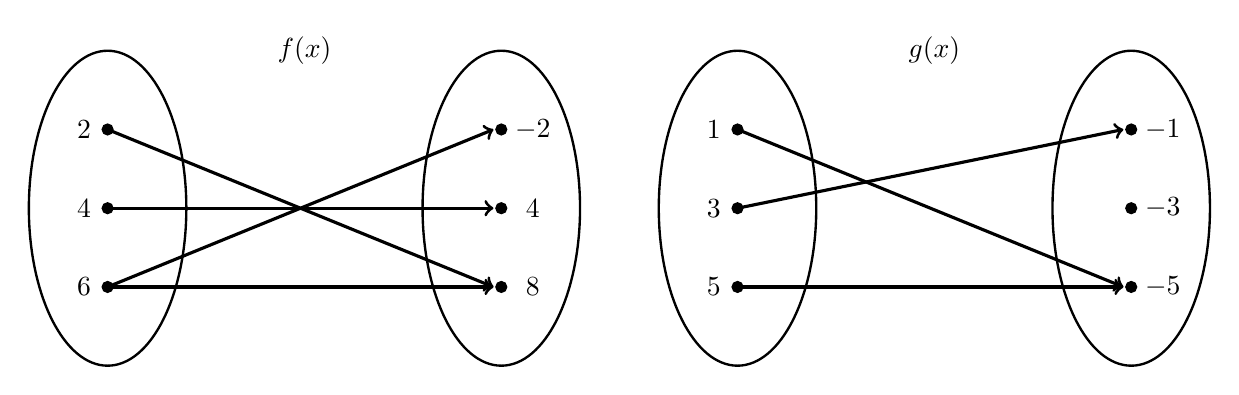
\begin{tikzpicture}
	\node at (2.5,2) {$f(x)$};
	% Ellipses
	\draw[line width=0.03cm] (0,0) circle (1 and 2);
	\draw[line width=0.03cm] (5,0) circle (1 and 2);
	
	% Nodes
	\draw[fill=black] (0,1) circle (0.07);
	\draw[fill=black] (0,0) circle (0.07);
	\draw[fill=black] (0,-1) circle (0.07);
	
	\draw[fill=black] (5,1) circle (0.07);
	\draw[fill=black] (5,0) circle (0.07);
	\draw[fill=black] (5,-1) circle (0.07);
	
	% Arrow
	\draw[line width=0.04cm,->] (0,1) -- (4.9,-1);
	\draw[line width=0.04cm,->] (0,0) -- (4.9,0);
	\draw[line width=0.04cm,->] (0,-1) -- (4.9,1);
	\draw[line width=0.04cm,->] (0,-1) -- (4.9,-1);
	
	% Labels
	\node at (-0.3,1) {$2$};
	\node at (-0.3,0) {$4$};
	\node at (-0.3,-1) {$6$};
	
	\node at (5.4,1) {$-2$};
	\node at (5.4,0) {$4$};
	\node at (5.4,-1) {$8$};
	
	\tikzset{shift={(8,0)}}
	%
	\node at (2.5,2) {$g(x)$};
	% Ellipses
	\draw[line width=0.03cm] (0,0) circle (1 and 2);
	\draw[line width=0.03cm] (5,0) circle (1 and 2);
	
	% Nodes
	\draw[fill=black] (0,1) circle (0.07);
	\draw[fill=black] (0,0) circle (0.07);
	\draw[fill=black] (0,-1) circle (0.07);
	
	\draw[fill=black] (5,1) circle (0.07);
	\draw[fill=black] (5,0) circle (0.07);
	\draw[fill=black] (5,-1) circle (0.07);
	
	% Arrow
	\draw[line width=0.04cm,->] (0,1) -- (4.9,-1);
	\draw[line width=0.04cm,->] (0,0) -- (4.9,1);
	\draw[line width=0.04cm,->] (0,-1) -- (4.9,-1);
	
	% Labels
	\node at (-0.3,1) {$1$};
	\node at (-0.3,0) {$3$};
	\node at (-0.3,-1) {$5$};
	
	\node at (5.4,1) {$-1$};
	\node at (5.4,0) {$-3$};
	\node at (5.4,-1) {$-5$};
	\end{tikzpicture}
	\]



\newpage



% Problem 2
\problem{10} Suppose $f(x)$ is the function given below.
	\[
	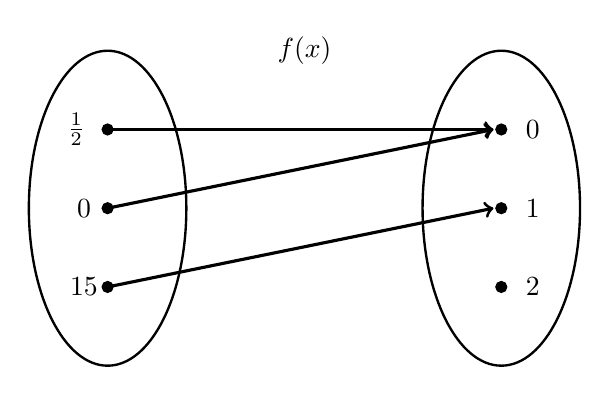
\begin{tikzpicture}
	\node at (2.5,2) {$f(x)$};
	% Ellipses
	\draw[line width=0.03cm] (0,0) circle (1 and 2);
	\draw[line width=0.03cm] (5,0) circle (1 and 2);
	
	% Nodes
	\draw[fill=black] (0,1) circle (0.07);
	\draw[fill=black] (0,0) circle (0.07);
	\draw[fill=black] (0,-1) circle (0.07);
	
	\draw[fill=black] (5,1) circle (0.07);
	\draw[fill=black] (5,0) circle (0.07);
	\draw[fill=black] (5,-1) circle (0.07);
	
	% Arrow
	\draw[line width=0.04cm,->] (0,1) -- (4.9,1);
	\draw[line width=0.04cm,->] (0,0) -- (4.9,1);
	\draw[line width=0.04cm,->] (0,-1) -- (4.9,0);
	
	% Labels
	\node at (-0.4,1) {$\frac{1}{2}$};
	\node at (-0.3,0) {$0$};
	\node at (-0.3,-1) {$15$};
	
	\node at (5.4,1) {$0$};
	\node at (5.4,0) {$1$};
	\node at (5.4,-1) {$2$};
	\end{tikzpicture}
	\]

\begin{enumerate}[(a)]
\item Explain why $f(x)$ is a function.
\item Find the value of $f(x)$ on each value in its domain. 
\item What is the domain of $f(x)$?
\item What is the codomain of $f(x)$?
\item What is the range of $f(x)$?
\end{enumerate}



\newpage



% Problem 3
\problem{10} Explain why $f(x, y)= 2x^2 - y^3 + 6$ is a function. Then find $f(0, 0)$, $f(3, -1)$, $f(-3, 2)$, and $f(1, 1)$. 



\newpage



% Problem 4
\problem{10} Give an example of a `real world' relationship between two variables which does represent a functional relationship. Also, give an example of a `real world' relationship between two variables which \textit{does not} represent a functional relationship. Be sure to fully explain your responses. 


\end{document}